% !TeX spellcheck = en_US
\chapter{Image Formation}
\label{cha:image-formation}

\section{Camera Obscura}
\ac{aka} the "Dark Chamber" (Leonardo Da Vinci, 1545)
\begin{figure}[hbt!]
	\centering
	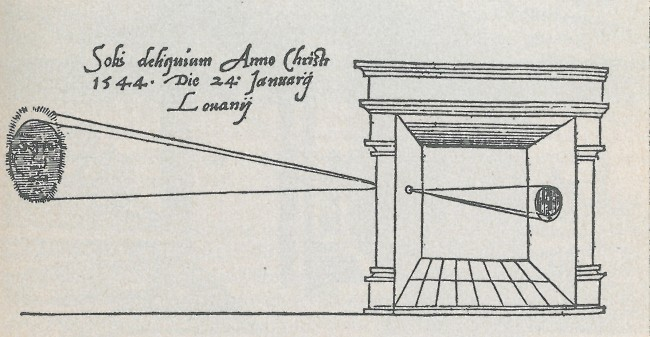
\includegraphics[width=0.79\textwidth]{camera-obscura.jpg}
	\caption{Camera obscura \cite{frisiusradio}.}
\end{figure}

\section{Pinhole Camera}
\begin{itemize}
	\item Pinhole size $=$ aperture
	\begin{itemize}
		\item too big $\Rightarrow$ blurring
		\item too small $\Rightarrow$ also blur, but because of diffraction\\ but then, \hlb{image is dark}
	\end{itemize}
	$\Rightarrow$ Use lenses: keep image sharp while \hlb{capture more light}
	\item The thin lens
	\item Focus \& Depth of Field:
	\begin{itemize}
		\item Large aperture: small depth of field\\
		(only object within the correct distance will be at focus, while background is blur)
		\item Small aperture: large depth of field, but need more light
	\end{itemize}
	\item The lens focus $f \gtrless$ field of view
	\begin{figure}[hbt!]
		\centering
		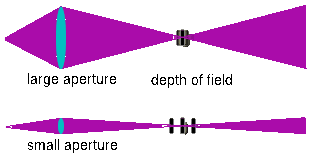
\includegraphics[width=0.57\textwidth]{depth-of-field.png}
		\caption{Varied depths of field depending on aperture size.}
	\end{figure}
	\begin{itemize}
		\item $f$ gets smaller $\Rightarrow$ wide-range image
		\item $f$ gets greater $\Rightarrow$ telescopic image
	\end{itemize}
\end{itemize}

\section{Digital image}
\begin{itemize}
	\item Discretize the image into a grid of pixels
	\item Quantize light intensities $\Rightarrow$ pixel values
	\item Resolution: \ac{no} pixels (most commonly understand)
\end{itemize}

\section{Color Sensing}
Referring to the process of assigning pixel values from color information of world objects.
\begin{itemize}
	\item Color image: RGB is just 1 of many color spaces, \eg, LUV, XYZ (\href{https://en.wikipedia.org/wiki/List_of_color_spaces_and_their_uses}{Wikipedia}).
	\item Grey-scale image
\end{itemize}

\subsection{Demosaicing}
Digital camera takes in light through a filter (Bayer or Xtrans) $\Rightarrow$ we get a gray-scale image (\figref{fig:demosaicing}). We need to apply demosaicing based on the filter's pattern to get the color image from the raw image. Sources: \href{https://www.youtube.com/watch?v=9cPxEFpg3Eg}{YouTube}, \href{https://en.wikipedia.org/wiki/Demosaicing}{Wikipedia}.
\begin{figure}[hbt!]
	\centering
	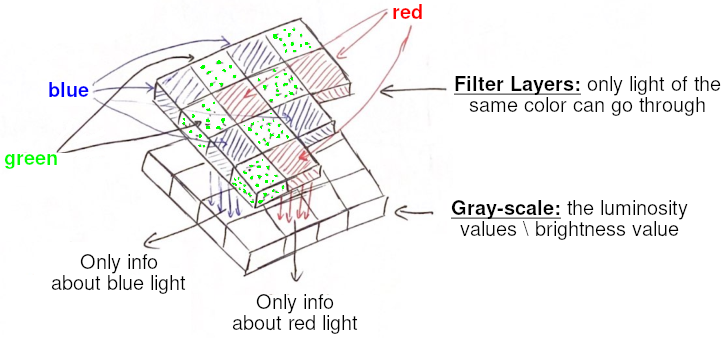
\includegraphics[width=\textwidth]{demosaicing.png}
	\caption{\Eg Bayer Filter. In the raw image , which lies below the filter layers, each pixel only has \ac{info} of only 1 among 3 light sources. Demosaicing uses the values of surrounding pixels to infer the brightness of other light sources.}
	\label{fig:demosaicing}
\end{figure}

\note Raw image has a \hlb{green cast}\\
Twice many green as red \& blue, because human eyes are twice as sensitive to the green part to other red or blue part.
